\section{Realizovaný rozvaděč s~elektronikou}
\begin{figure}[H]
   \centering
   \def\svgwidth{0.5\columnwidth}
   \input{images/svg/otopna-soustava/vyrez-rozvadec.pdf_tex}
    \caption[Umístění rozvaděče s elektronikou.]{Výřez z obrázku \ref{fig:otopna-soustava-a-elektronika-rez-domu}. Umístění rozvaděče s elektronikou.}
    \label{fig:vyrez-rozvadec}
\end{figure}

Na obrázku \ref{fig:vyrez-rozvadec} je výřez části z celkového nákresu (obrázek \ref{fig:otopna-soustava-a-elektronika-rez-domu}) systému znázorňující umístění rozvaděče s elektronikou. V realizovaném rozvaděči na obrázku \ref{fig:rozvadec-ve-sklepe-s-elektronikou} je umístěn 5 V zdroj pro napájení centrální jednotky, relé modulů, I$^2$C diferenciální sběrnice, napájení 1-Wire sběrnice, napájení elektroniky u krbů a napájení pro zónové regulátory. Dále je zde 12 V zdroj pro napájení dvou chodbových termostatů. Zdroj 24 V pro zónové regulátory, respektive pro napájení termoelektrických pohonů. V  neposlední řadě jsou zde jističe pro jednotlivé zdroje a čerpadla včetně proudového chrániče.

\begin{figure}[H]
    \centering
    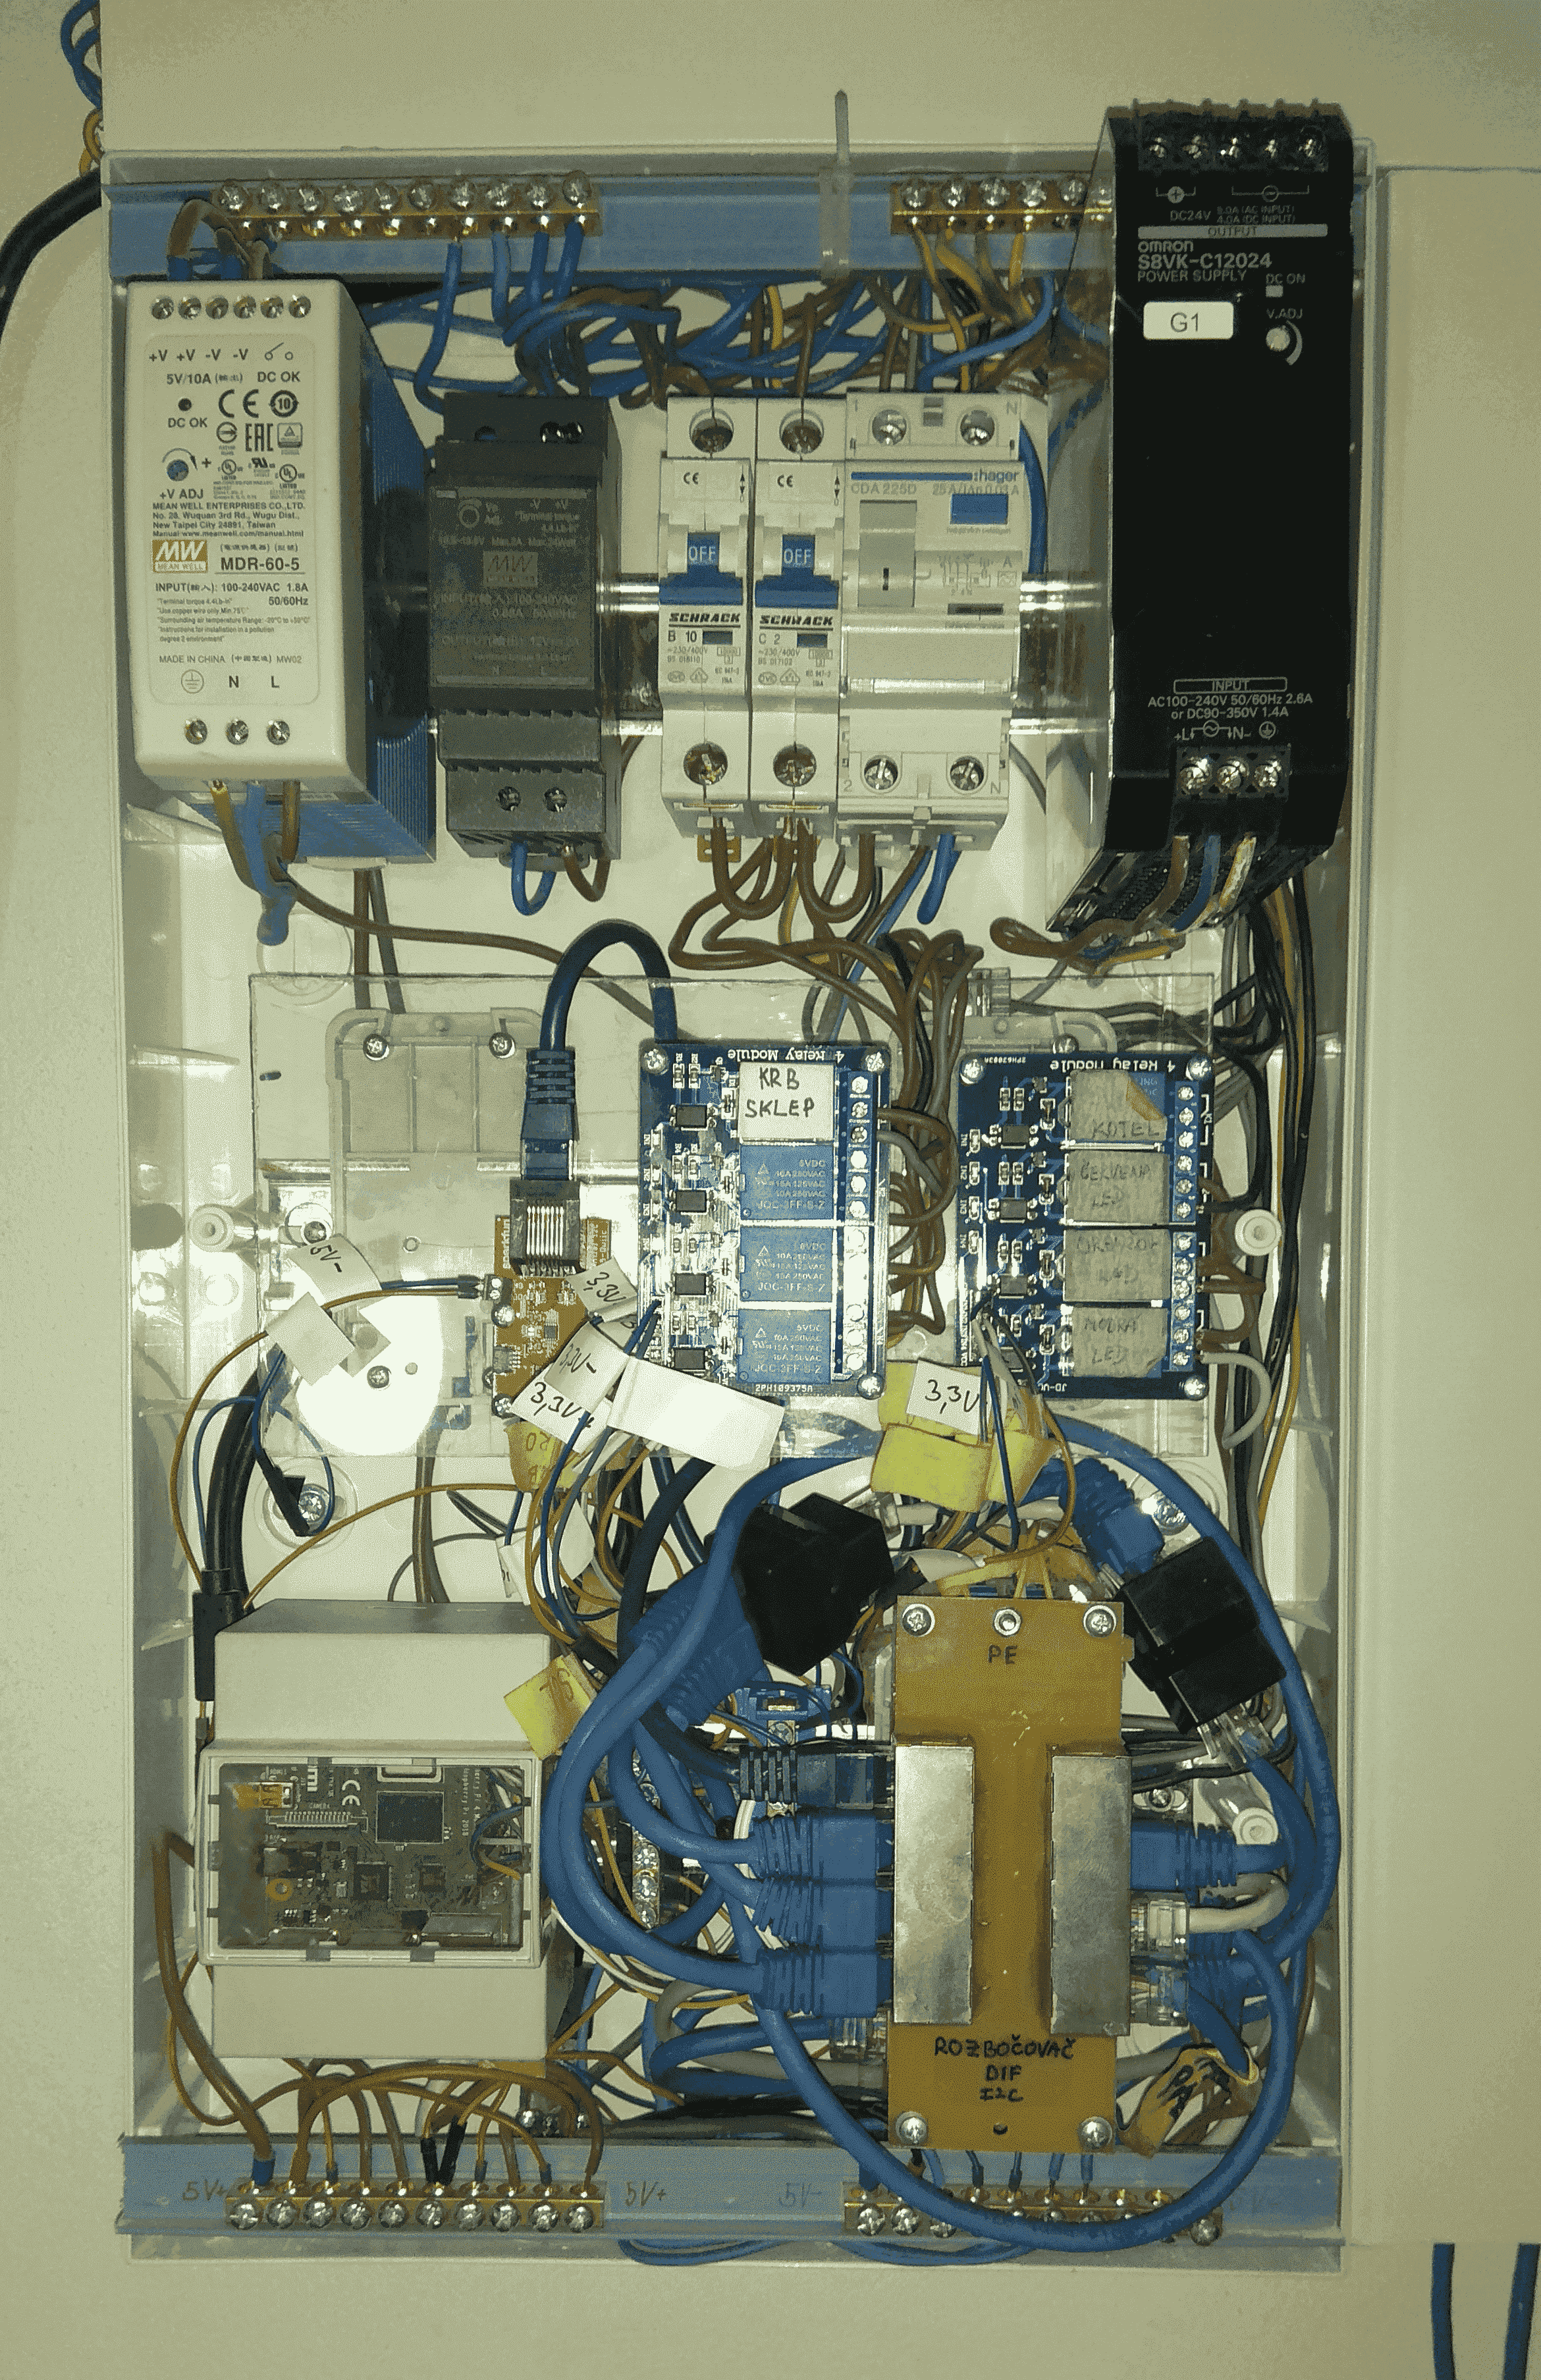
\includegraphics[width=\textwidth]{images/rozvadec-ve-sklepe-s-elektronikou.png}
    \caption{Realizovaný rozvaděč s~elektronikou.}
    \label{fig:rozvadec-ve-sklepe-s-elektronikou}
\end{figure}